\documentclass{beamer}

\usepackage{bookmark}

\title{Deep Neural Network for Real-Time EEG Decoding of Musical Rhythm Imagery}
\author{Ir\'{a}n Rom\'{a}n}
\date{December 03, 2019}

\begin{document}
\setbeamertemplate{caption}{\raggedright\insertcaption\par}

\maketitle

\begin{frame}
	\frametitle{Pulse and Meter as Neural Resonance}
	
	\begin{itemize}

		\item Pulse: (aka beat) the repeating, periodic \textit{pulsation} 
			that we \textit{perceive} through time when we listen to music
		\begin{itemize}
			\item Tempo: the pulse's frequency over time
		\end{itemize}

		\item Meter: The patterns of accentuation between pulses (i.e. march or waltz)

		\item Neural Resonance: Music can trigger rhythmic bursts of high-frequency neural activity,
			 which may enable communication between auditory and motor cortices (Large \& Snyder 2009)

	\end{itemize}

\end{frame}

\begin{frame}
	\frametitle{Early EEG Evidence for Neural Resonance}

	Induced and evoked oscilatory activity reflect the processing and expectation of periodic stimuli

	\begin{figure}
		\centering
		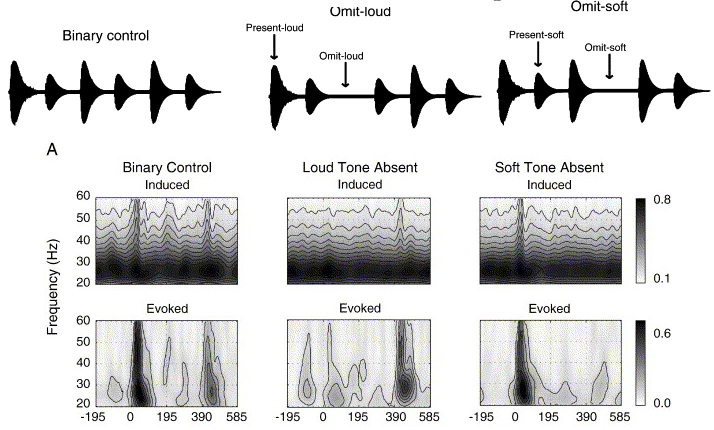
\includegraphics[scale=2.5]{fig1.png}
		\caption{Snyder \& Large 2005}
	\end{figure}

\end{frame}

\begin{frame}
	\frametitle{Pulse timing is reflected in beta- and gamma-bands}

	\begin{figure}
		\centering
		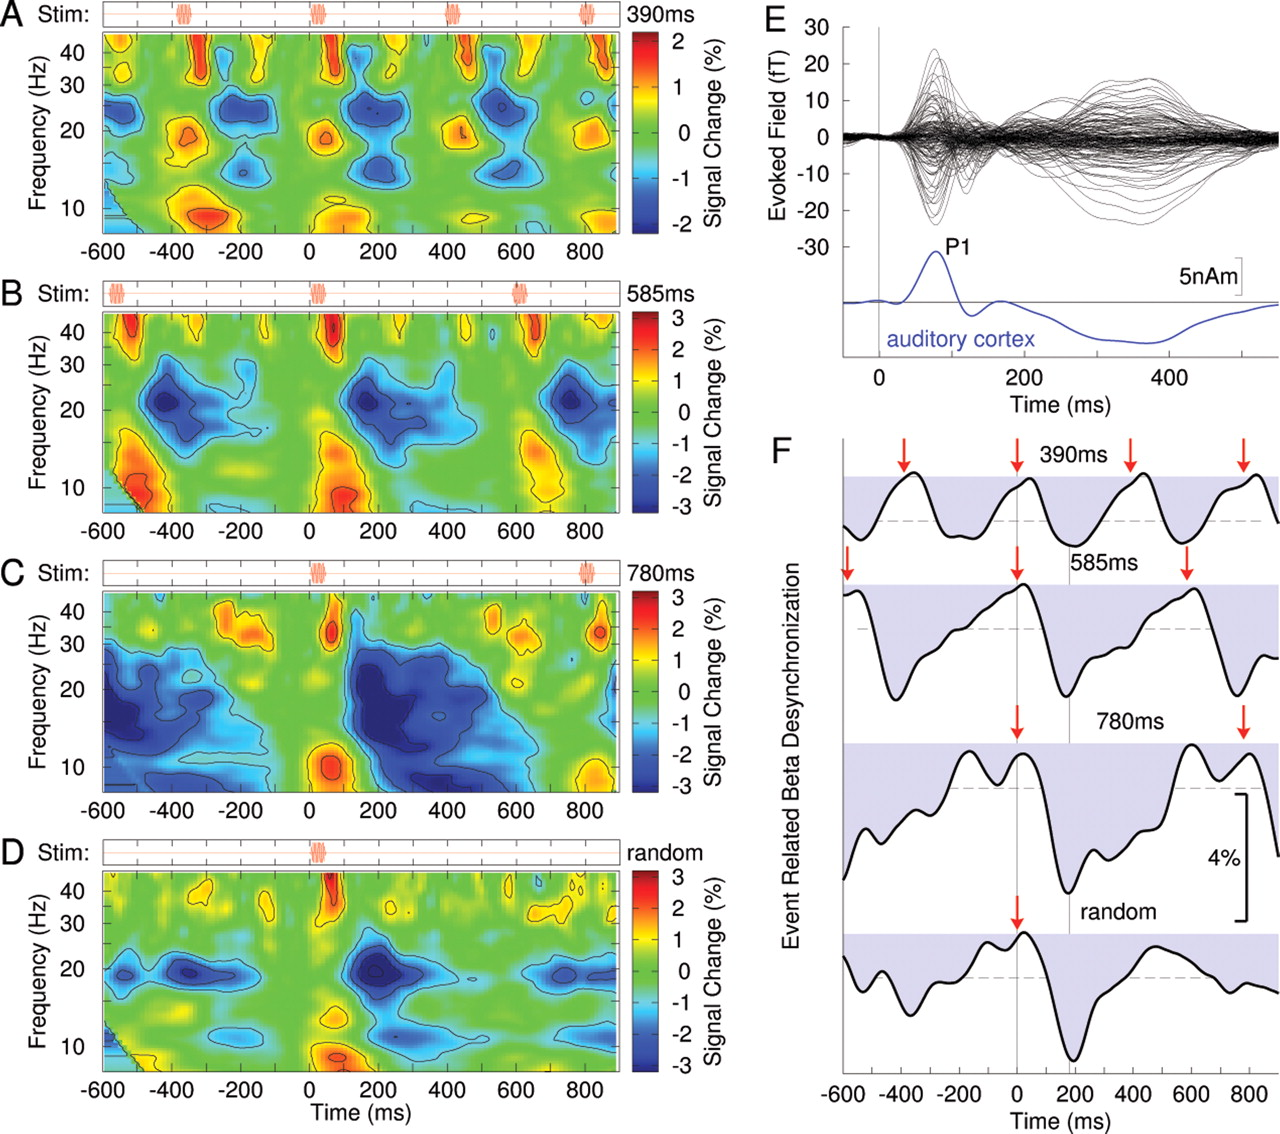
\includegraphics[scale=0.18]{fig5.jpg}
		\caption{Fujioka et al. 2009}
	\end{figure}

\end{frame}

\begin{frame}
	\frametitle{Pulse timing is reflected in beta- and gamma-bands}

	\begin{figure}
		\centering
		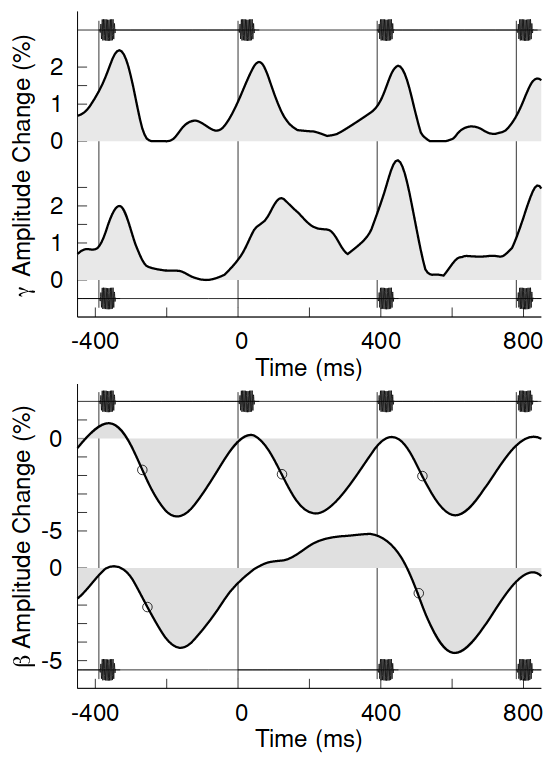
\includegraphics[scale=0.2]{fig2.png}
		\caption{Fujioka et al. 2012}
	\end{figure}

	This kind of analysis involves the averaging of hundreds of trials

\end{frame}

\begin{frame}
	\frametitle{Imagined meters are also reflected in the beta-band}

	Imagination of different meters (i.e. binary march vs ternary waltz) results in different beta-band patterns

	\begin{figure}
		\centering
		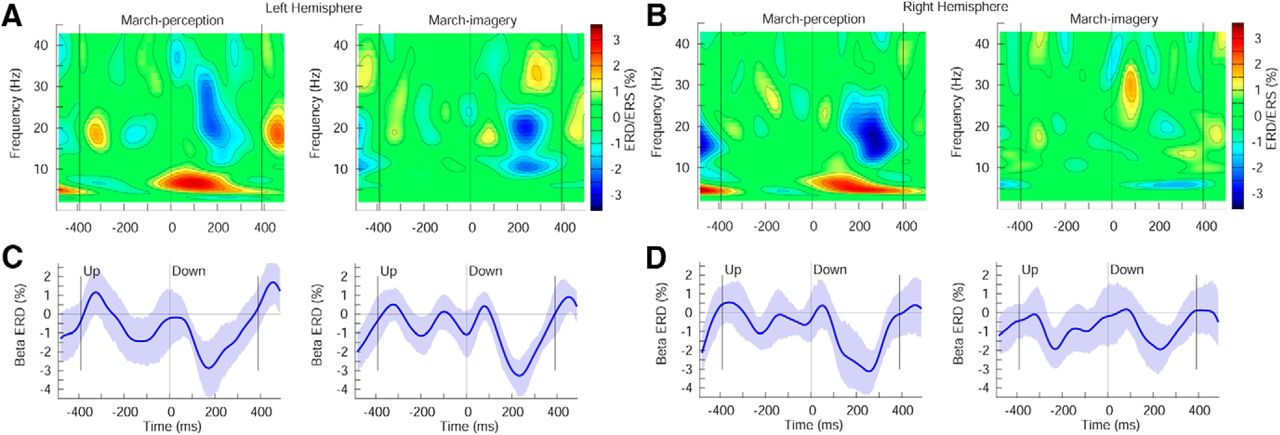
\includegraphics[scale=0.85]{fig3.jpg}
	\end{figure}
	\begin{figure}
		\centering
		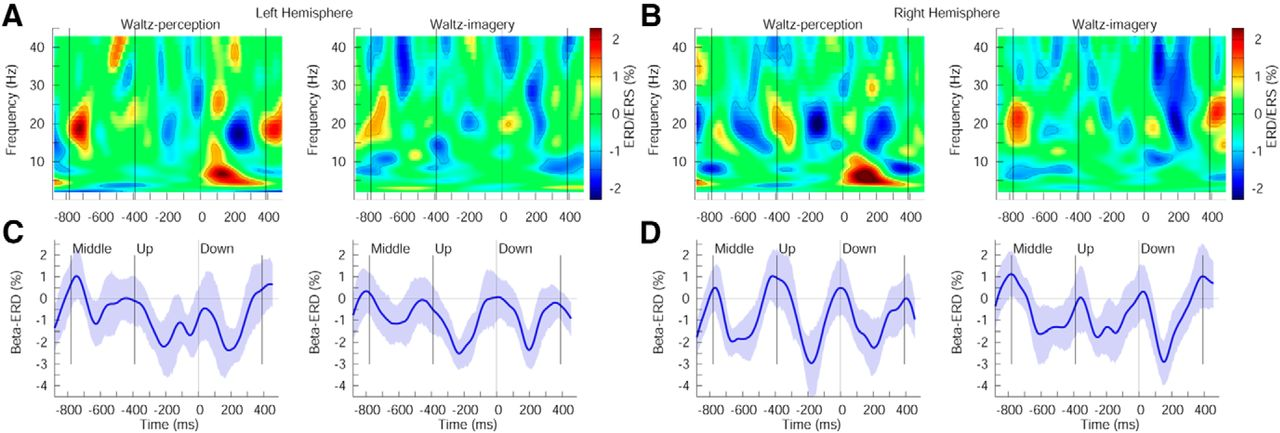
\includegraphics[scale=0.85]{fig4.jpg}
		\caption{Fujioka et al. 2015}
	\end{figure}

\end{frame}

\begin{frame}
	\frametitle{Primate oscillations reflect the metronome tempo}

	Dorsal putamen LFPs of macaques in a metronome tapping task	

	\begin{figure}
		\centering
		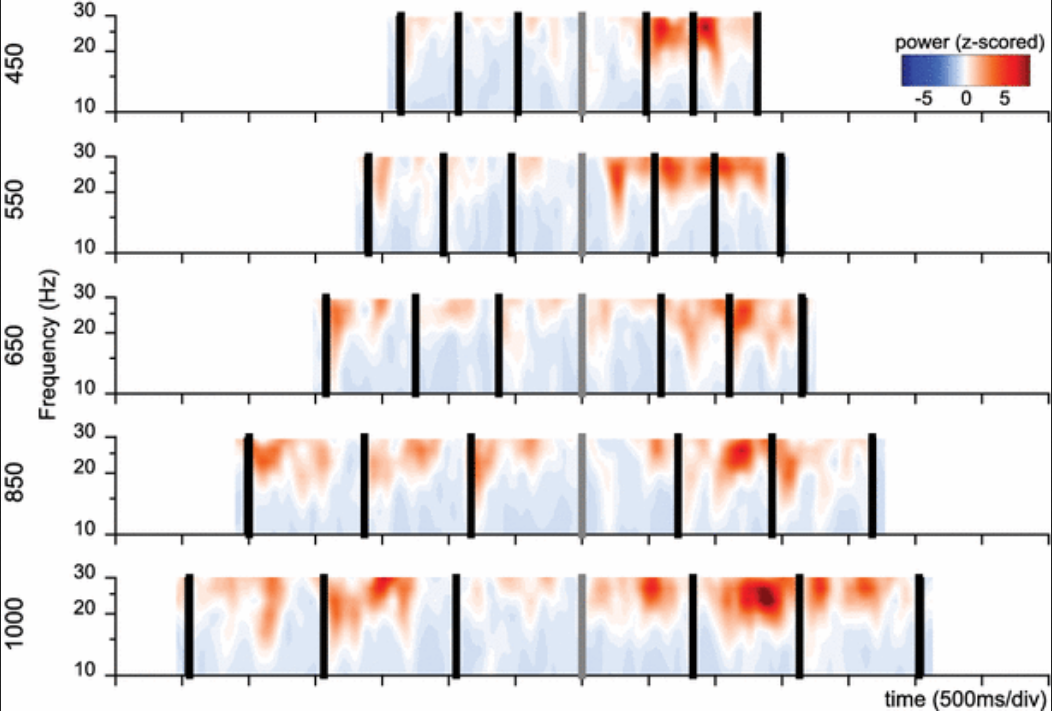
\includegraphics[scale=0.18]{fig6.png}
		\caption{Merchant \& Bartolo 2017}
	\end{figure}

	Bottomline: gamma reflects stimulus processing, while beta reflects the entrainment of large basal ganglia networks during internally driven pulse tapping

\end{frame}

\begin{frame}
	\frametitle{Research question and hypothesis}
	
	\begin{itemize}

		\item Pulse, tempo and meter can be observed in the neural correlates measured with EEG and MEG.

		\item To maximize the SNR, these observations require the analysis of hundreds of trials.

		\item \textbf{Research Question:} could these features be identified in single trials? and if so, can we decode from human brain data, in real-time, perceived and imagined musical features like pulse, tempo and meter? 
			 
		\item \textbf{Hypothesis:} Deep neural networks, like CNNs, can learn to identify these musical features on a single-trial level.

	\end{itemize}

\end{frame}

\end{document}
